%\vspace{\sectionReduceTop}
\section{VQA Baselines and Methods}
%\vspace{\sectionReduceBot}
\begin{figure*}[h]
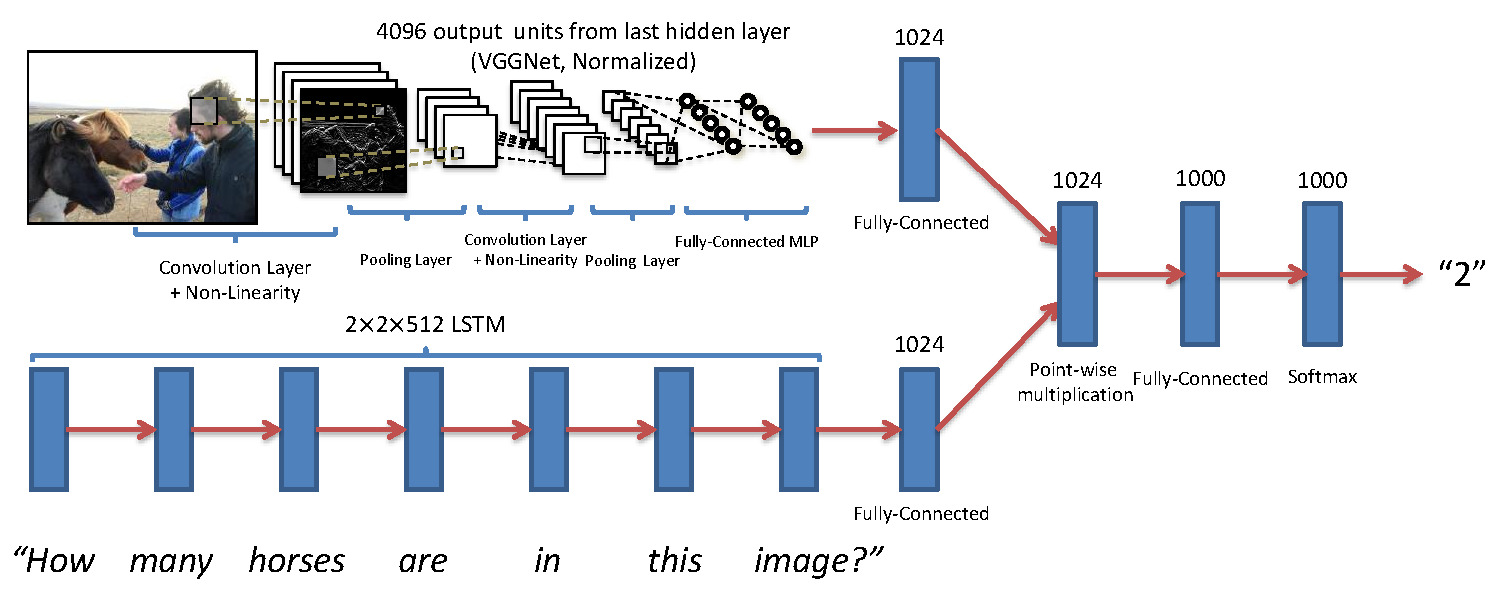
\includegraphics[width=1\linewidth]{figures/best_model_compressed.pdf}
\centering
\caption{Our best performing model (deeper LSTM Q + norm I). This model uses a two layer LSTM to encode the questions and the last hidden layer of VGGNet~\cite{Simonyan14c} to encode the images. The image features are then $\ell_2$ normalized. Both the question and image features are transformed to a common space and fused via element-wise multiplication, which is then passed through a fully connected layer followed by a softmax layer to obtain a distribution over answers.}
\label{fig:best_model}
%\vspace{\captionReduceBot}
\end{figure*}
In this section, we explore the difficulty of the VQA dataset for the MS COCO images using several baselines 
and novel methods. We train on VQA train+val. Unless stated otherwise, all human accuracies are on test-standard, machine accuracies are on test-dev, and results involving human captions (in gray font) are trained on train and tested on val (because captions are not available for test). 

\subsection{Baselines}
\label{sec:baselinesmain}
We implemented the following baselines:
\begin{enumerate}
\item \textbf{random:} We randomly choose an answer from the top 1K answers of the VQA train/val dataset.

\item \textbf{prior (``yes''):} We always select the most popular answer (``yes'') for both the open-ended and multiple-choice tasks. Note that ``yes'' is always one of the choices for the multiple-choice questions.

\item \textbf{per Q-type prior:} For the open-ended task, we pick the most popular answer per question type (see the appendix for details). For the multiple-choice task, we pick the answer (from the provided choices) that is most similar to the picked answer for the open-ended task using cosine similarity in Word2Vec\cite{word2vec} feature space.

\item \textbf{nearest neighbor:} Given a test image, question pair, we first find the $K$ nearest neighbor questions and associated images from the training set. See appendix for details on how neighbors are found. Next, for the open-ended task, we pick the most frequent ground truth answer from this set of nearest neighbor question, image pairs. Similar to the ``per Q-type prior'' baseline, for the multiple-choice task, we pick the answer (from the provided choices) that is most similar to the picked answer for the open-ended task using cosine similarity in \\ Word2Vec\cite{word2vec} feature space.
\end{enumerate}

%If we randomly choose an answer from the top 1K answers of the VQA train/val dataset, 
%the test-standard accuracy is $0.12\%$. 
%If we always select the most popular answer (``yes''), the accuracy is $29.72\%$. Picking the most popular answer per question type does $37.55\%$ and a nearest neighbor approach does $42.73\%$ on test-standard (see the appendix for details).
%For testing, we use the same train/val/test splits as COCO$^2$. 
%we split our real image dataset into a training and testing dataset. Our training dataset contains $30,000$ images and our testing dataset contains $20,000$ images. \jiasen{change image numbers, also including the NN baseline?}
\vspace{-5pt}
\subsection{Methods}
\label{sec:methods}
For our methods, we develop a 2-channel vision (image) + language (question) model that culminates with a softmax over $K$ possible outputs. We choose the top $K = 1000$ most frequent answers as possible outputs. This set of answers covers $82.67\%$ of the train+val answers. We describe the different components of our model below:

\textbf{Image Channel:} This channel provides an embedding for the image. We experiment with two embeddings -- 
\begin{compactenum}
\item \textbf{I:} The activations from the last hidden layer of VGGNet~\cite{Simonyan14c} are used as 4096-dim image embedding.
\item \textbf{norm I:} These are $\ell_2$ normalized activations from the last hidden layer of VGGNet~\cite{Simonyan14c}.
\end{compactenum}

\textbf{Question Channel:} This channel provides an embedding for the question. We experiment with three embeddings --
\begin{compactenum}
\item \textbf{Bag-of-Words Question (BoW Q)}: The top 1,000 words in the questions are used to create a bag-of-words representation. Since there is a strong correlation between the words that start a question and the answer (see \figref{fig:AnsPerQues}), we find the top 10 first, second, and third words of the questions and create a 30 dimensional bag-of-words representation. These features are concatenated to get a 1,030-dim embedding for the question.
\item \textbf{LSTM Q:} An LSTM with one hidden layer is used to obtain 1024-dim embedding for the question. The embedding obtained from the LSTM is a concatenation of last cell state and last hidden state representations (each being 512-dim) from the hidden layer of the LSTM. Each question word is encoded with 300-dim embedding by a fully-connected layer + tanh non-linearity which is then fed to the LSTM. The input vocabulary to the embedding layer consists of all the question words seen in the training dataset.
\item \textbf{deeper LSTM Q:} An LSTM with two hidden layers is used to obtain 2048-dim embedding for the question. The embedding obtained from the LSTM is a concatenation of last cell state and last hidden state representations (each being 512-dim) from each of the two hidden layers of the LSTM. Hence 2 (hidden layers) x 2 (cell state and hidden state) x 512 (dimensionality of each of the cell states, as well as hidden states) in \figref{fig:best_model}. This is followed by a fully-connected layer + tanh non-linearity to transform 2048-dim embedding to 1024-dim. The question words are encoded in the same way as in LSTM Q.   
\end{compactenum}

\textbf{Multi-Layer Perceptron (MLP):} The image and question embeddings 
%obtained from the image and question channels respectively 
are combined to obtain a single embedding. 
\begin{compactenum}
\item For \textbf{BoW Q + I} method, we simply concatenate the BoW Q and I embeddings. 
\item For \textbf{LSTM Q + I}, and \textbf{deeper LSTM Q + norm I} (\figref{fig:best_model}) methods, the image embedding is first transformed to 1024-dim by a fully-connected layer + tanh non-linearity to match the LSTM embedding of the question. The transformed image and LSTM embeddings (being in a common space) are then fused via element-wise multiplication. 
\end{compactenum}
This combined image + question embedding is then passed to an MLP -- a fully connected neural network classifier with 2 hidden layers and 1000 hidden units (dropout 0.5) in each layer with tanh non-linearity, followed by a softmax layer to obtain a distribution over $K$ answers. The entire model is learned end-to-end with a cross-entropy loss. VGGNet parameters are frozen to those learned for ImageNet classification and not fine-tuned in the image channel.   

We also experimented with providing captions as input to our model. Similar to \tableref{table:commonsense_acc}, we assume that a human-generated caption is given as input. We use a bag-of-words representation containing the 1,000 most popular words in the captions as the caption embedding (\textbf{Caption}). For \textbf{BoW Question + Caption (BoW Q + C)} method, we simply concatenate the BoW Q and C embeddings. 
%\jiasen{We don't know the coverage on test set, should we report the coverage on train+val set?} All baselines train a softmax neural network classifier with a single hidden layer containing 50 units. \jiasen{We have MLP baseline and LSTM baseline. For the MLP baseline, we train a softmax neural network classifier with 2 hidden layer each containing 1000 units. We use Tanh() as non-linear function and apply Dropout with probability 0.5 in each hidden layer.} 
%We experiment with three models: 
%(i) a multi-layer perceptron (MLP) neural network classifier with 2 hidden layers and 1000 hidden 
%units (dropout 0.5) in each layer with tanh non-linearity,  
%(ii) an LSTM model followed by a softmax layer to obtain a distribution over answers, and
%(iii) a two layer deeper LSTM model followed by softmax layer to obtain a distribution over answers.
%We experimented with five inputs for the MLP model. \textbf{Bag-of-Words Question (BoW Q)}: The top 1,000 words in the questions are used to create a bag-of-words representation. Since there is a strong correlation between the words that start a question and the answer (see \figref{fig:AnsPerQues}), we find the top 10 first, second, and third words of the questions and create a 30 dimensional bag-of-words representation. These features are concatenated to get a 1,030 dimensional input representation. \textbf{Caption:} Similar to \tableref{table:commonsense_acc}, we assume that a human-generated caption is given as input. We use a bag-of-words representation containing the 1,000 most popular words in the captions as the input feature. \textbf{Image (I):} We use the last hidden layer of VGGNet~\cite{Simonyan14c} as our 4096-dim feature. We also report the learned baseline results on \textbf{BoW Question + Image (BoW Q + I)} and \textbf{BoW Question + Caption (BoW Q + C)} by simply concatenating the first hidden layer representations of networks trained on each feature individually. The LSTM model uses a one-hot encoding for the question words, and the same image features as above followed by a linear + tanh transformation to transform the image features to 1024 dimensions to match the LSTM encoding of the question. The question and image encodings are fused via element-wise multiplication. The deeper LSTM Q model uses two hidden layers in the LSTM unlike only one hidden layer in the LSTM model. The deeper LSTM Q + norm I model (\figref{fig:best_model}) has almost the same architecture as the LSTM Q + I model except that it uses deeper LSTM (two hidden layer) and $l2$ normalized image features.

%For LSTM question only baseline, we simply input the question words into the LSTM along and fed into a softmax layer at the last timestep to generate the answers. For the LSTM vis baseline, we use the same VGG Conv Net fc7 layer feature, and use a linear trainsforamtion to map 4096 dimension image feature vectors to 1024 dimensional vector that match the dimension of encoded question feature. We fuse the image and question feature by doing an element-wise multiplication and further fed into a softmax layer. } 
For testing, we report the result on two different tasks: open-ended selects the answer with highest activation from all possible $K$ answers and multiple-choice picks the answer that has the highest activation from the potential answers. 

\subsection{Results}
\label{sec:results}

\begin{table}[t] \scriptsize
\setlength{\tabcolsep}{1.8pt}
\begin{center}
\begin{tabular}{@{} l  c  c  c  c  c  c c c@{}}
%\hline
\toprule
& \multicolumn{4}{c}{Open-Ended} & \multicolumn{4}{c}{ Multiple-Choice} \\

\cmidrule[0.75pt](l){2-5}
\cmidrule[0.75pt](l){6-9}
 & All & Yes/No & Number & Other & All & Yes/No & Number & Other \\
%\hline
\midrule
prior (``yes'') & 29.66 & 70.81 & 00.39 & 01.15 & 29.66 & 70.81 & 00.39 & 01.15 \\
per Q-type prior & 37.54 & 71.03 & 35.77 & 09.38 &  39.45 & 71.02 & 35.86 & 13.34 \\
nearest neighbor & 42.70 & 71.89 & 24.36 & 21.94 & 48.49 & 71.94 & 26.00 & 33.56 \\
BoW Q & \textcolor{black}{48.09} & \textcolor{black}{75.66} &  \textcolor{black}{36.70}& \textcolor{black}{27.14} 
& \textcolor{black}{53.68} & \textcolor{black}{75.71} & \textcolor{black}{37.05} & \textcolor{black}{38.64}\\
I & \textcolor{black}{28.13} & \textcolor{black}{64.01} & 00.42 & \textcolor{black}{03.77}  
&\textcolor{black}{30.53} & \textcolor{black}{69.87} & 00.45 & \textcolor{black}{03.76}\\
BoW Q + I & \textcolor{black}{52.64} & \textcolor{black}{75.55} & 33.67 & \textcolor{black}{37.37} 
& \textcolor{black}{58.97} & \textcolor{black}{75.59} & 34.35 & \textcolor{black}{50.33}\\
LSTM Q & \textcolor{black}{48.76} & \textcolor{black}{78.20} & 35.68 & \textcolor{black}{26.59} 
& \textcolor{black}{54.75} & \textcolor{black}{78.22} & 36.82 &\textcolor{black}{38.78}\\
LSTM Q + I & \textcolor{black}{53.74} & \textcolor{black}{78.94} & 35.24 & \textcolor{black}{36.42} 
& \textcolor{black}{57.17} & \textcolor{black}{78.95}& 35.80 & \textcolor{black}{43.41}\\
deeper LSTM Q & \textcolor{black}{50.39} & \textcolor{black}{78.41} & 34.68 & \textcolor{black}{30.03} 
& \textcolor{black}{55.88} & \textcolor{black}{78.45} & 35.91 &\textcolor{black}{41.13}\\
%\textcolor{red}{deeper LSTM Q} \\
deeper LSTM Q + norm I & \textbf{57.75} & \textbf{80.50} & \textbf{36.77} & \textbf{43.08} 
& \textbf{62.70} & \textbf{80.52}& \textbf{38.22} & \textbf{53.01}\\
%\textcolor{red}{norm I} \\
\midrule
\textcolor{gray}{Caption} & \textcolor{gray}{26.70} & \textcolor{gray}{65.50} & \textcolor{gray}{02.03} & \textcolor{gray}{03.86} 
& \textcolor{gray}{28.29} & \textcolor{gray}{69.79} & \textcolor{gray}{02.06} & \textcolor{gray}{03.82}\\
\textcolor{gray}{BoW Q + C} & \textcolor{gray}{54.70} & \textcolor{gray}{75.82} & \textcolor{gray}{40.12} & \textcolor{gray}{42.56} 
& \textcolor{gray}{59.85} & \textcolor{gray}{75.89} & \textcolor{gray}{41.16}  & \textcolor{gray}{52.53}\\
\bottomrule
\end{tabular}	
\caption{Accuracy of our methods for the open-ended and multiple-choice tasks on the VQA test-dev for real images. 
Q = Question, I = Image, C = Caption. (Caption and BoW Q + C results are on val). 
See text for details.
}
%\vspace{-10pt}
\label{tab:acc}
\end{center}
\end{table}
\tableref{tab:acc} shows the accuracy of our baselines and methods for both the open-ended and multiple-choice tasks on the VQA test-dev for real images.

As expected, the vision-alone model (I) that completely ignores the question performs rather poorly (open-ended: 28.13\% / multiple-choice: 30.53\%). In fact, on open-ended task, the vision-alone model (I) performs worse than the prior (``yes'') baseline, which ignores both the image \emph{and} question (responding to every question with a ``yes''). 

Interestingly, the language-alone methods (per Q-type prior, BoW Q, LSTM Q) that ignore the image perform surprisingly well, with BoW Q achieving 48.09\% on open-ended (53.68\% on multiple-choice) and LSTM Q achieving 48.76\% on open-ended (54.75\% on multiple-choice); both outperforming the nearest neighbor baseline (open-ended: 42.70\%, multiple-choice: 48.49\%). Our quantitative results and analyses suggest that this might be due to the language-model exploiting subtle statistical priors about the question types (e.g. ``What color is the banana?'' can be answered with ``yellow'' without looking at the image). For a detailed discussion of the subtle biases in the questions, please see \cite{yinyang}. 

The accuracy of our \textbf{best model} (deeper LSTM Q + norm I (\figref{fig:best_model}), selected using VQA test-dev accuracies) on VQA test-standard is 58.16\% (open-ended) / 63.09\% (multiple-choice). We can see that our model is able to significantly outperform both the vision-alone and language-alone baselines. As a general trend, results on multiple-choice are better than open-ended. All methods are significantly worse than human performance.
%The accuracy of our \textbf{best model} (deeper LSTM Q + norm I (\figref{fig:best_model}), selected using VQA test-dev accuracies) on VQA test-standard is $\textbf{58.16\%}$.
%The accuracy using only the question is $\sim$48\%, which demonstrates that the type of question is informative of the answer. As expected, results on multiple-choice are better than open-ended. 
%%In comparison to 
%All methods are significantly worse than human performance. 

Our VQA demo is available on CloudCV \cite{cloudcv} -- \url{http://cloudcv.org/vqa}. This will be updated with newer models as we develop them.

%\textcolor{red}{In \tableref{tab:acc}, the results of (Q + I) are very similar to the results of only using the questions, while the addition of captions (Q + C) provides minimal improvement $\sim2-4\%$.} 
To gain further insights into these results, we computed accuracies by question type in \tableref{tab:typeacc}. Interestingly, for question types that require more reasoning, such as ``Is the'' or ``How many'', the scene-level image features do not provide any additional information. However, for questions that can be answered using scene-level information, such as ``What sport,'' 
%or ``What animal''
we do see an improvement. Similarly, for questions whose answer may be contained in a generic caption we see improvement, such as ``What animal''. For all question types, the results are worse than human accuracies.

We also analyzed the accuracies of our best model (deeper LSTM Q + norm I) on a subset of questions with certain specific (ground truth) answers. In \figref{fig:prob_1}, we show the average accuracy of the model on questions with 50 most frequent ground truth answers on the VQA validation set (plot is sorted by accuracy, not frequency). We can see that the model performs well for answers that are common visual objects such as ``wii'', ``tennis'', ``bathroom'' while the performance is somewhat underwhelming for counts (\eg, ``2'', ``1'', ``3''), and particularly poor for higher counts (\eg, ``5'', ``6'', ``10'', ``8'', ``7''). 

In \figref{fig:prob_2}, we show the distribution of 50 most frequently predicted answers when the system is correct on the VQA validation set (plot is sorted by prediction frequency, not accuracy). In this analysis, ``system is correct'' implies that it has VQA accuracy $1.0$ (see section \ref{sec:dataset} for accuracy metric). We can see that the frequent ground truth answers (\eg, ``yes'', ``no'', ``2'', ``white'', ``red'', ``blue'', ``1'', ``green'') are more frequently predicted than others when the model is correct. 

%This observation suggests that the model is probably learning the distribution of answers in the training dataset.

%%%%%%%%%%%%%%%%%%%%%%%%%%%%%%%%%%%%%%%%%%%%%%%%%%%%%%%%%


\begin{table}[h] \scriptsize
\setlength{\tabcolsep}{2pt}
\begin{center}
\begin{tabular}{@{} l  c  c  c  c c c c@{}  }
%\hline
\toprule
& \multicolumn{5}{c}{Open-Ended}   & Human Age & Commonsense\\

%\cline{2-6}
\cmidrule[0.9pt](l){2-6}

\multicolumn{1}{c}{Question} & \multicolumn{3}{c}{K = 1000} & \multicolumn{2}{c}{Human} & To Be Able & To Be Able\\
\cmidrule[0.5pt](lr){2-4}
\cmidrule[0.5pt](l){5-6}

\multicolumn{1}{c}{Type}  & Q & Q + I & Q + C & Q & Q + I & To Answer & To Answer (\%)\\
%\hline
\midrule
what is \textcolor{black}{(13.84)} & \textcolor{black}{23.57} & \textcolor{black}{34.28} & \textcolor{gray}{43.88} & \textcolor{black}{16.86} & \textcolor{black}{73.68} &\textcolor{black}{09.07} & 27.52\\
what color \textcolor{black}{(08.98)} & \textcolor{black}{33.37} & \textcolor{black}{43.53} & \textcolor{gray}{48.61} & \textcolor{black}{28.71} & \textcolor{black}{86.06} &\textcolor{black}{06.60} & 13.22\\
what kind \textcolor{black}{(02.49)} & \textcolor{black}{27.78} & \textcolor{black}{42.72} & \textcolor{gray}{43.88} & \textcolor{black}{19.10} & \textcolor{black}{70.11} &\textcolor{black}{10.55} & 40.34\\
what are \textcolor{black}{(02.32)} & \textcolor{black}{25.47} & \textcolor{black}{39.10} & \textcolor{gray}{47.27} & \textcolor{black}{17.72} & \textcolor{black}{69.49} &\textcolor{black}{09.03} & 28.72\\
what type \textcolor{black}{(01.78)} & \textcolor{black}{27.68} & \textcolor{black}{42.62} & \textcolor{gray}{44.32} & \textcolor{black}{19.53} & \textcolor{black}{70.65} &\textcolor{black}{11.04} & 38.92\\
is the \textcolor{black}{(10.16)} & \textcolor{black}{70.76} & \textcolor{black}{69.87} & \textcolor{gray}{70.50} & \textcolor{black}{65.24} & \textcolor{black}{95.67} &\textcolor{black}{08.51} & 30.30\\
is this \textcolor{black}{(08.26)} & \textcolor{black}{70.34} & \textcolor{black}{70.79} & \textcolor{gray}{71.54} & \textcolor{black}{63.35} & \textcolor{black}{95.43} &\textcolor{black}{10.13} & 45.32\\
how many \textcolor{black}{(10.28)} & \textcolor{black}{43.78} & \textcolor{black}{40.33} & \textcolor{gray}{47.52} & \textcolor{black}{30.45} & \textcolor{black}{86.32} &\textcolor{black}{07.67}& 15.93 \\
are \textcolor{black}{(07.57)} & \textcolor{black}{73.96} & \textcolor{black}{73.58} & \textcolor{gray}{72.43} & \textcolor{black}{67.10} & \textcolor{black}{95.24} &\textcolor{black}{08.65} & 30.63\\
does \textcolor{black}{(02.75)} & \textcolor{black}{76.81} & \textcolor{black}{75.81} & \textcolor{gray}{75.88} & \textcolor{black}{69.96} & \textcolor{black}{95.70} &\textcolor{black}{09.29} & 38.97\\
where \textcolor{black}{(02.90)} & \textcolor{black}{16.21} & \textcolor{black}{23.49} & \textcolor{gray}{29.47} & \textcolor{black}{11.09} & \textcolor{black}{43.56} &\textcolor{black}{09.54} & 36.51\\
is there \textcolor{black}{(03.60)} & \textcolor{black}{86.50} & \textcolor{black}{86.37} & \textcolor{gray}{85.88} & \textcolor{black}{72.48} & \textcolor{black}{96.43} &\textcolor{black}{08.25} & 19.88\\
why \textcolor{black}{(01.20)} & \textcolor{black}{16.24} & \textcolor{black}{13.94} & \textcolor{gray}{14.54} & \textcolor{black}{11.80} & \textcolor{black}{21.50} &\textcolor{black}{11.18} & 73.56\\
which \textcolor{black}{(01.21)} & \textcolor{black}{29.50} & \textcolor{black}{34.83} & \textcolor{gray}{40.84} & \textcolor{black}{25.64} & \textcolor{black}{67.44} &\textcolor{black}{09.27} & 30.00\\
do \textcolor{black}{(01.15)} & \textcolor{black}{77.73} & \textcolor{black}{79.31} & \textcolor{gray}{74.63} & \textcolor{black}{71.33} & \textcolor{black}{95.44} &\textcolor{black}{09.23} & 37.68\\
what does \textcolor{black}{(01.12)} & \textcolor{black}{19.58} & \textcolor{black}{20.00} & \textcolor{gray}{23.19} & \textcolor{black}{11.12} & \textcolor{black}{75.88} &\textcolor{black}{10.02} & 33.27\\
what time \textcolor{black}{(00.67)} & \textcolor{black}{8.35} & \textcolor{black}{14.00} & \textcolor{gray}{18.28} & \textcolor{black}{07.64} & \textcolor{black}{58.98} &\textcolor{black}{09.81} & 31.83\\
who \textcolor{black}{(00.77)} & \textcolor{black}{19.75} & \textcolor{black}{20.43} & \textcolor{gray}{27.28} & \textcolor{black}{14.69} & \textcolor{black}{56.93} &\textcolor{black}{09.49} & 43.82\\
what sport \textcolor{black}{(00.81)} & \textcolor{black}{37.96} & \textcolor{black}{81.12} & \textcolor{gray}{93.87} & \textcolor{black}{17.86} & \textcolor{black}{95.59} &\textcolor{black}{08.07} & 31.87\\
what animal \textcolor{black}{(00.53)} & \textcolor{black}{23.12} & \textcolor{black}{59.70} & \textcolor{gray}{71.02} & \textcolor{black}{17.67} & \textcolor{black}{92.51} &\textcolor{black}{06.75} & 18.04\\
what brand \textcolor{black}{(00.36)} & \textcolor{black}{40.13} & \textcolor{black}{36.84} & \textcolor{gray}{32.19} & \textcolor{black}{25.34} & \textcolor{black}{80.95} &\textcolor{black}{12.50} & 41.33\\
                                                                                                                                                             
\bottomrule
\end{tabular}
\caption{Open-ended test-dev results for different question types on real images (Q+C is reported on val).
Machine performance is reported using the bag-of-words representation for questions.
Questions types are determined by the one or two words that start the question. 
The percentage of questions for each type is shown in parentheses. 
%All results are the percentage of answers in agreement with human subjects. 
Last and second last columns respectively show the average human age and average degree of commonsense required to answer the questions 
(as reported by AMT workers), respectively. 
See text for details.}
\vspace{-10pt}
\label{tab:typeacc}
\end{center}
\end{table}
%%%%%%%%%%%%%%%%%%%%%%%%%%%%%%%%%%%%%%%%%%%%%%%%%%%%%%%%%

%We also tested our baselines on only binary $K=2$ (\ie, ``yes/no'' questions). The results are shown in \tableref{tab:acc} (right column). The results generally improve upon the baseline of answering ``yes'' to every question (\textcolor{red}{$66.97\%$}). However, they are again significantly worse than human performance.

Finally, evaluating our best model (deeper LSTM Q + norm I) on the validation questions for which we have age annotations (how old a human needs to be to answer the question correctly), we estimate that our model performs as well as a $4.74$ year old child! The average age required on the same set of questions is $8.98$. Evaluating the same model on the validation questions for which we have commonsense annotations (whether the question requires commonsense to answer it), we estimate that it has degree of commonsense of $17.35\%$. The average degree of commonsense required on same set of questions is $31.23\%$. Again, these estimates reflect the age and commonsense perceived by MTurk workers that would be required to answer the question. See the appendix for details. 

We further analyzed the performance of the model for different age groups on the validation questions for which we have age annotations. In \figref{fig:age_1}, we computed the average accuracy of the predictions made by the model for questions belonging to different age groups. Perhaps as expected, the accuracy of the model decreases as the age of the question increases (from $61.07\%$ at $3-4$ age group to $47.83\%$ at $18+$ age group). 

In \figref{fig:age_2}, we show the distribution of age of questions for different levels of accuracies achieved by our system on the validation questions for which we have age annotations. It is interesting to see that the relative proportions of different age groups is consistent across all accuracy bins with questions belonging to the age group 5-8 comprising the majority of the predictions which is expected because 5-8 is the most common age group in the dataset (see \figref{fig:age}).

%\begin{figure*}[t]
%\includegraphics[width=1\linewidth]{figures/prob1_sorted_pvalues_OpenEnded_val2014.pdf}
%\centering
%\caption{$\Pr\text{(system is correct }|\text{ answer\_i)}$ for 50 most accurate answers.}
%\label{fig:prob_1_sorted_pvalues}
%%\vspace{\captionReduceBot}
%\end{figure*}
\begin{figure*}[h]
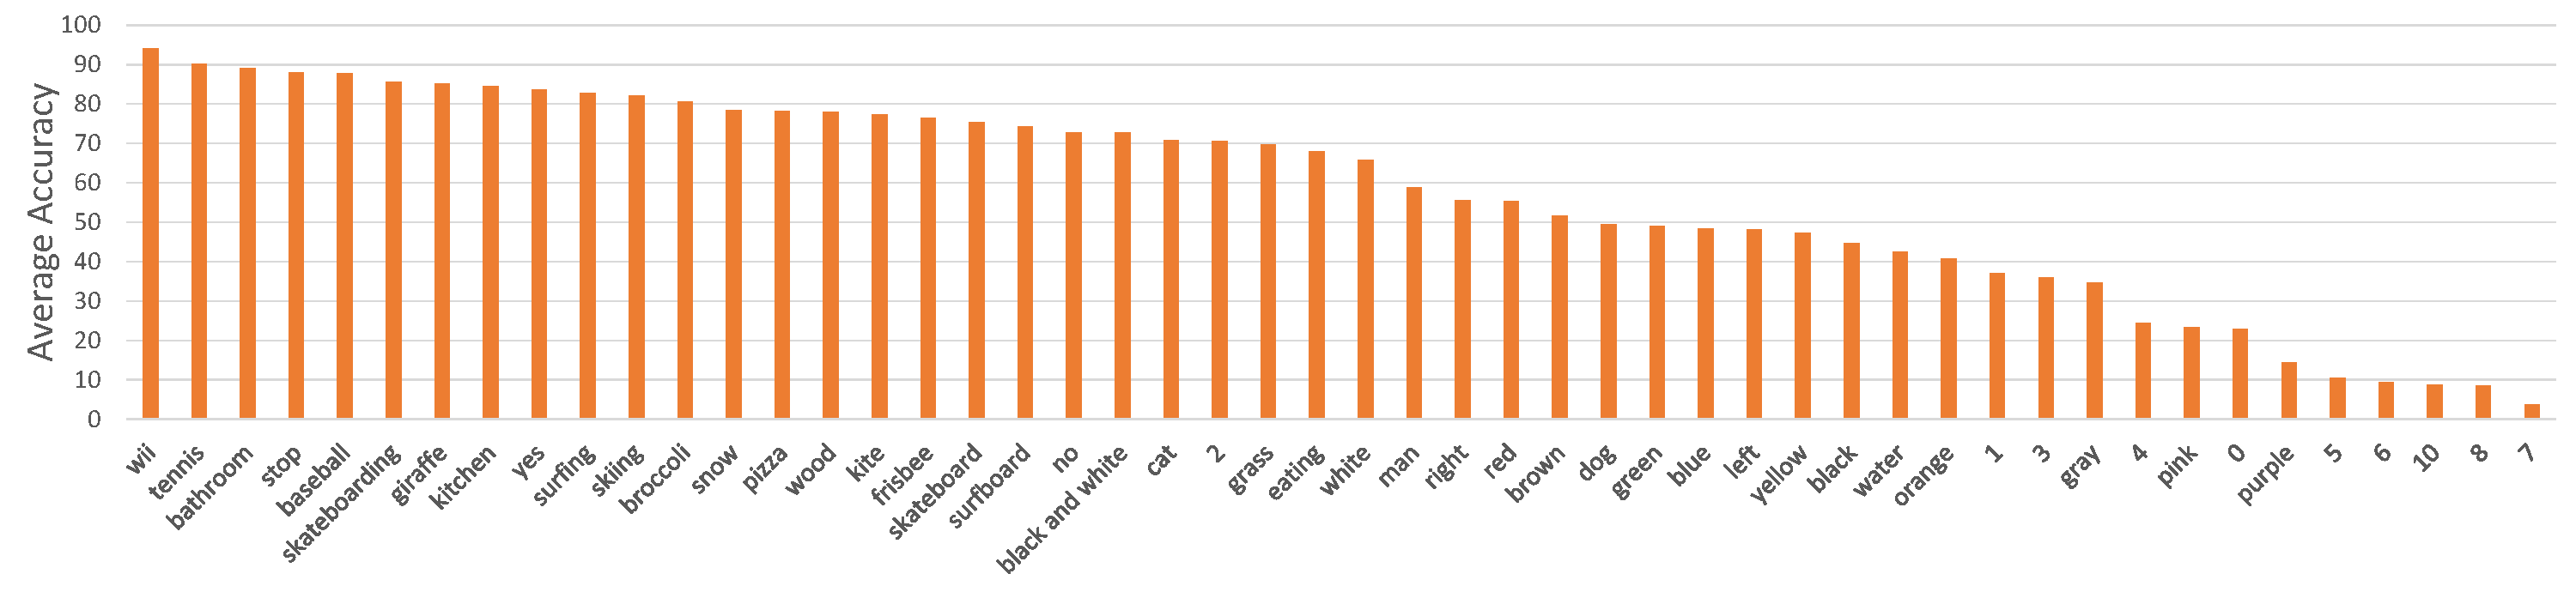
\includegraphics[width=1\linewidth]{figures/prob1_OpenEnded_val2014_sorted.pdf}
\centering
\caption{$\Pr\text{(system is correct } | \text{ answer)}$ for 50 most frequent ground truth answers on the VQA validation set (plot is sorted by accuracy, not frequency). System refers to our best model (deeper LSTM Q + norm I).}
\label{fig:prob_1}
%\vspace{\captionReduceBot}
\end{figure*}
\begin{figure*}[h]
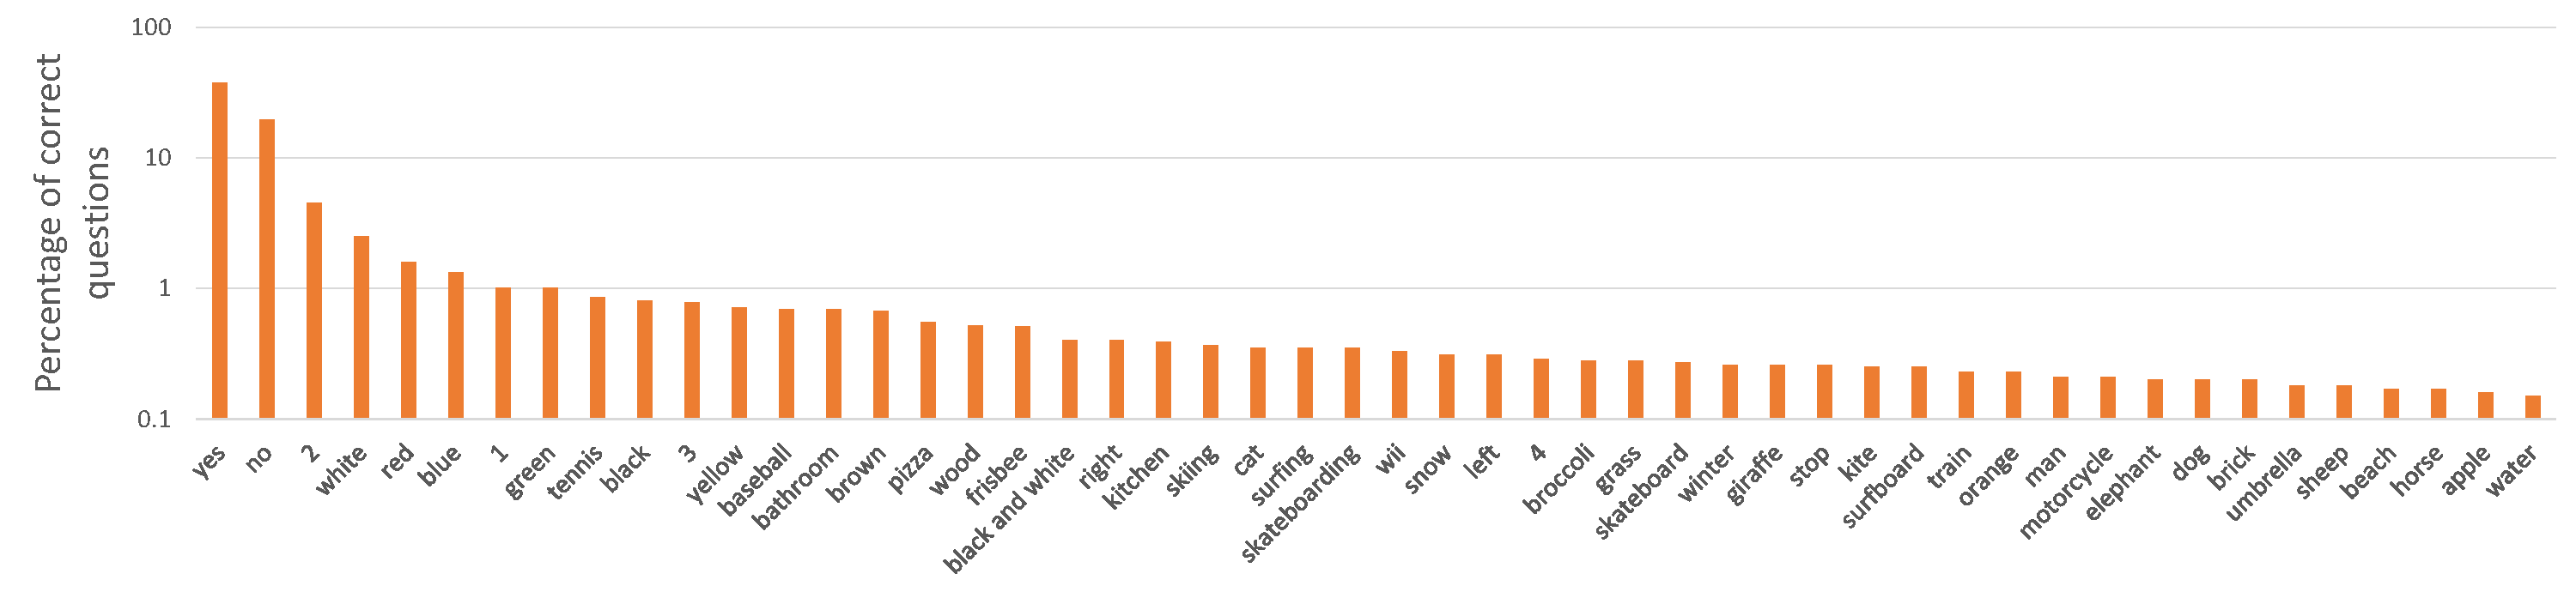
\includegraphics[width=1\linewidth]{figures/prob2_OpenEnded_val2014_100_logscale.pdf}
\centering
\caption{$\Pr\text{(answer } | \text{ system is correct)}$ for 50 most frequently predicted answers on the VQA validation set (plot is sorted by prediction frequency, not accuracy). System refers to our best model (deeper LSTM Q + norm I).}
\label{fig:prob_2}
%\vspace{\captionReduceBot}
\end{figure*}
\begin{figure}[h]
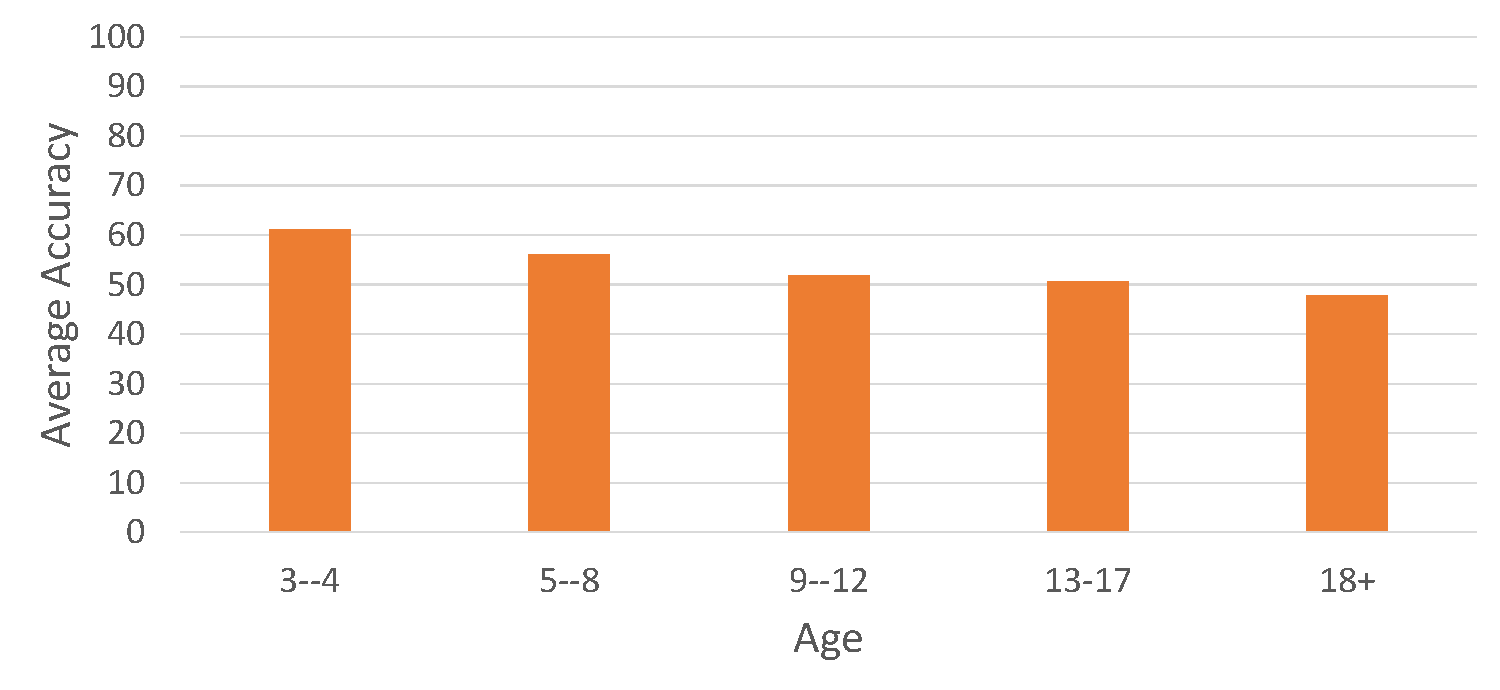
\includegraphics[width=1\linewidth]{figures/OpenEnded_val2014_predAgeDict2.pdf}
\centering
\caption{$\Pr\text{(system is correct } | \text{ age of question)}$ on the VQA validation set. System refers to our best model (deeper LSTM Q + norm I).}
\label{fig:age_1}
%\vspace{\captionReduceBot}
\end{figure}
\begin{figure}[h]
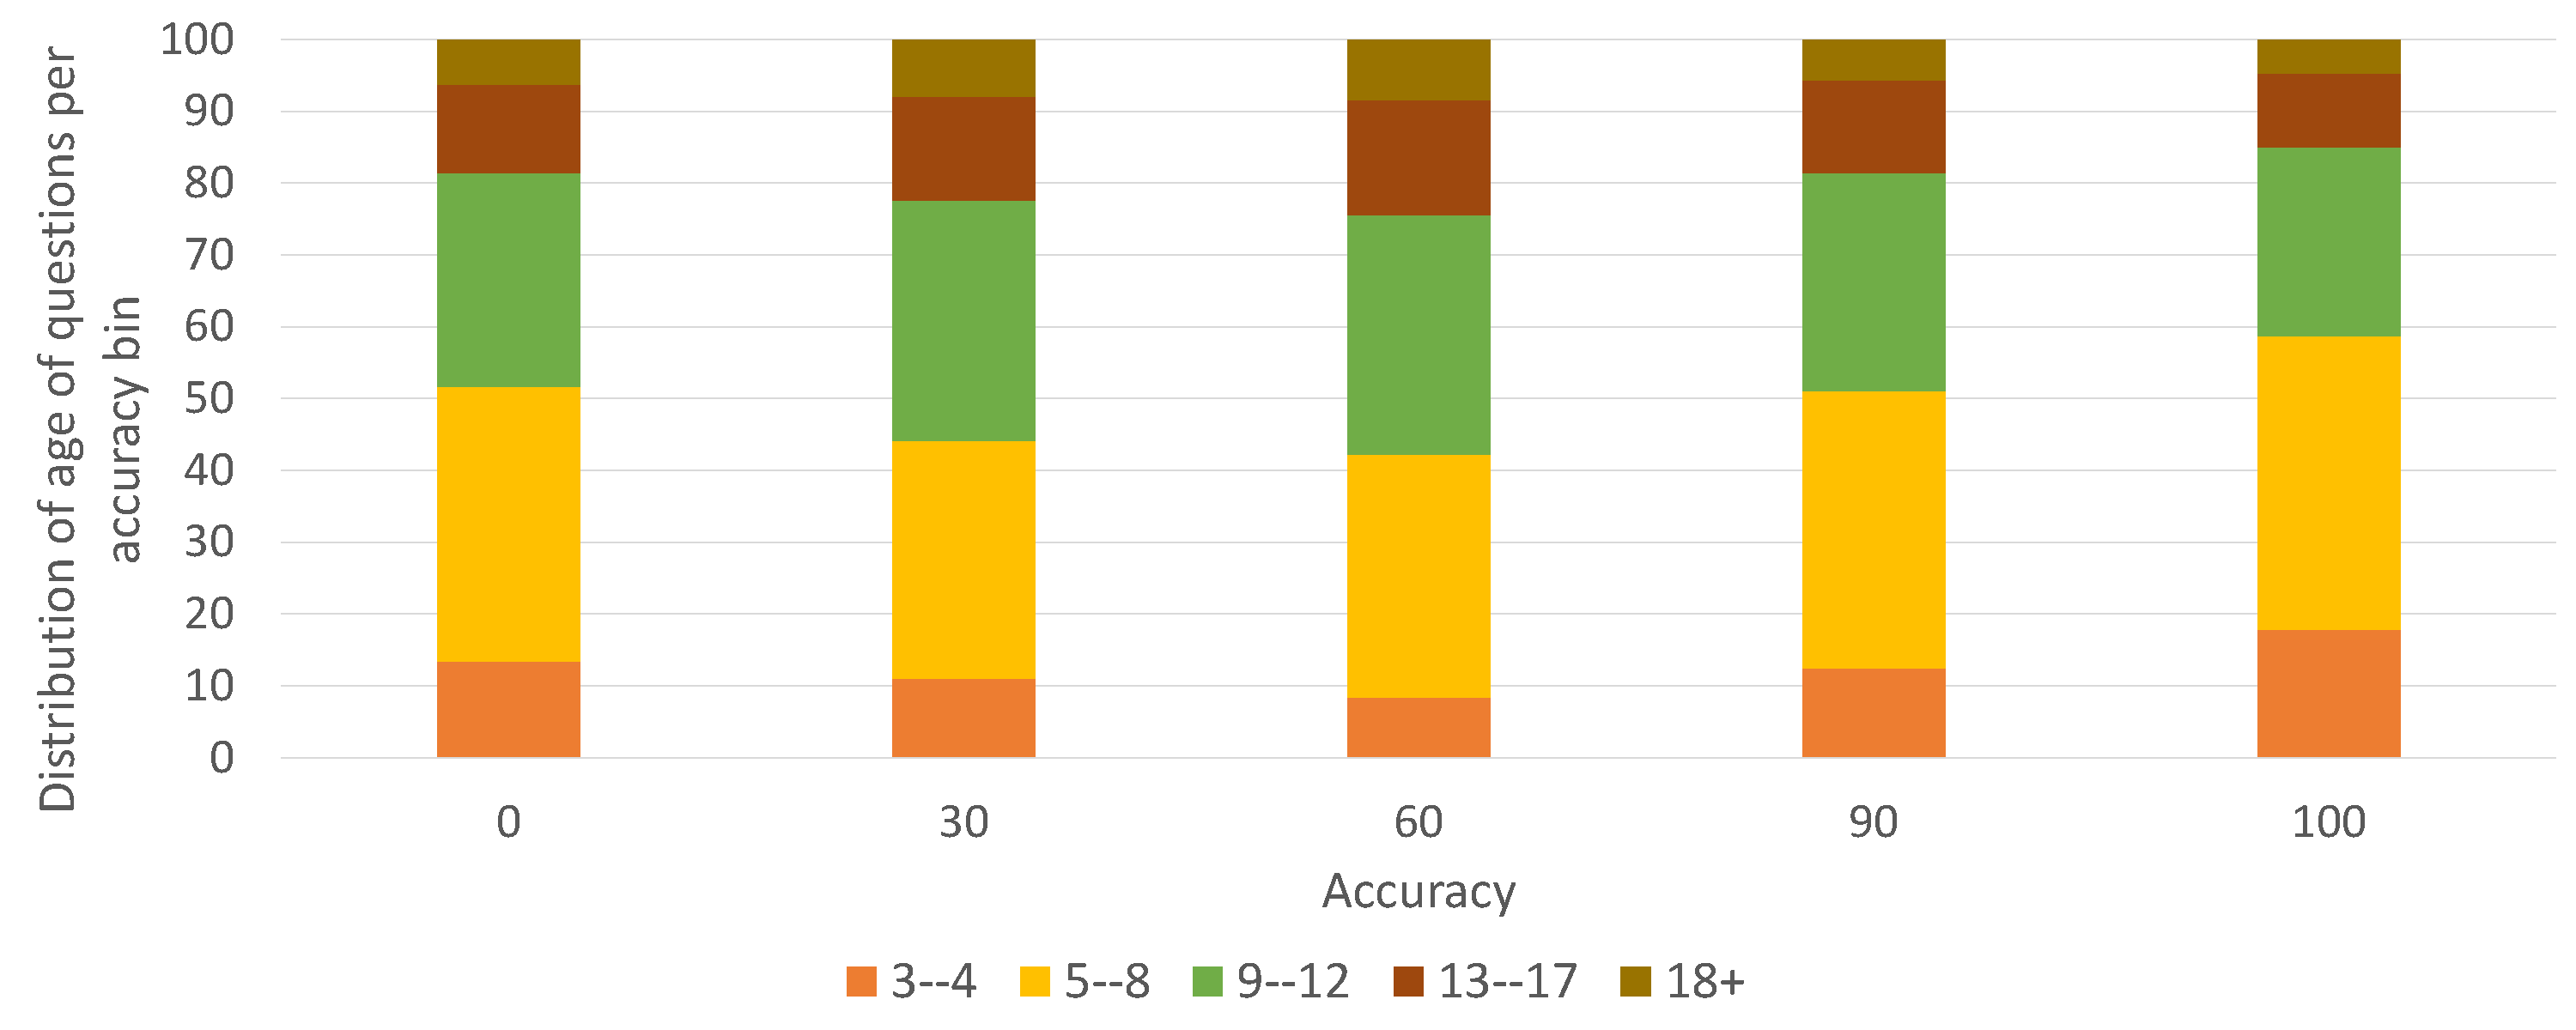
\includegraphics[width=1\linewidth]{figures/OpenEnded_val2014_predAgeDict1.pdf}
\centering
\caption{$\Pr\text{(age of question } | \text{ system is correct)}$ on the VQA validation set. System refers to our best model (deeper LSTM Q + norm I).}
\label{fig:age_2}
%\vspace{\captionReduceBot}
\end{figure}

\tableref{tab:abl_acc} shows the accuracy of different ablated versions of our best model (deeper LSTM Q + norm I) for both the open-ended and multiple-choice tasks on the VQA test-dev for real images. The different ablated versions are as follows --

\begin{compactenum}
\item \textbf{Without I Norm:} In this model, the activations from the last hidden layer of VGGNet~\cite{Simonyan14c} are not $\ell_2$-normalized. Comparing the accuracies in \tableref{tab:abl_acc} and \tableref{tab:acc}, we can see that $\ell_2$-normalization of image features boosts the performance by 0.16\% for open-ended task and by 0.24\% for multiple-choice task. 

\item \textbf{Concatenation:} In this model, the transformed image and LSTM embeddings are concatenated (instead of element-wise multiplied), resulting in doubling the number of parameters in the following fully-connected layer. Comparing the accuracies in \tableref{tab:abl_acc} and \tableref{tab:acc}, we can see that element-wise fusion performs better by 0.95\% for open-ended task and by 1.24\% for multiple-choice task.

\item \textbf{K = 500:} In this model, we use K = 500 most frequent answers as possible outputs. Comparing the accuracies in \tableref{tab:abl_acc} and \tableref{tab:acc}, we can see that K = 1000 performs better than K = 500 by 0.82\% for open-ended task and by 1.92\% for multiple-choice task.

\item \textbf{K = 2000:} In this model, we use K = 2000 most frequent answers as possible outputs. Comparing the accuracies in \tableref{tab:abl_acc} and \tableref{tab:acc}, we can see that K = 2000 performs better then K = 1000 by 0.40\% for open-ended task and by 1.16\% for multiple-choice task.

\item \textbf{Truncated Q Vocab $@$ 5:} In this model, the input vocabulary to the embedding layer (which encodes the question words) consists of only those question words which occur atleast 5 times in the training dataset, thus reducing the vocabulary size from 14770 (when all question words are used) to 5134 (65.24\% reduction). Remaining question words are replaced with UNK (unknown) tokens. Comparing the accuracies in \tableref{tab:abl_acc} and \tableref{tab:acc}, we can see that truncating the question vocabulary $@$ 5 performs better than using all questions words by 0.24\% for open-ended task and by 0.17\% for multiple-choice task.

\item \textbf{Truncated Q Vocab $@$ 11:} In this model, the input vocabulary to the embedding layer (which encodes the question words) consists of only those question words which occur atleast 11 times in the training dataset, thus reducing the vocabulary size from 14770 (when all question words are used) to 3561 (75.89\% reduction). Remaining question words are replaced with UNK (unknown) tokens. Comparing the accuracies in \tableref{tab:abl_acc} and \tableref{tab:acc}, we can see that truncating the question vocabulary $@$ 11 performs better than using all questions words by 0.06\% for open-ended task and by 0.02\% for multiple-choice task.

\item \textbf{Filtered Dataset:} We created a filtered version of the VQA train + val dataset in which we only keep the answers with subject confidence ``yes''. Also, we keep only those questions for which at least 50\% (5 out of 10) answers are annotated with subject confidence ``yes''. The resulting filtered dataset consists of 344600 questions, compared to 369861 questions in the original dataset, thus leading to only 6.83\% reduction in the size of the dataset. The filtered dataset has 8.77 answers per question on average. We did not filter the test set so that accuracies of the model trained on the filtered dataset can be compared with that of the model trained on the original dataset. The row ``Filtered Dataset'' in \tableref{tab:abl_acc} shows the performance of the deeper LSTM Q + norm I model when trained on the filtered dataset. Comparing these accuracies with the corresponding accuracies in \tableref{tab:acc}, we can see that the model trained on filtered version performs worse by 1.13\% for open-ended task and by 1.88\% for multiple-choice task.
\end{compactenum}

\begin{table}[t] \scriptsize
\setlength{\tabcolsep}{1.8pt}
\begin{center}
\begin{tabular}{@{} l  c  c  c  c  c  c c c@{}}
%\hline
\toprule
& \multicolumn{4}{c}{Open-Ended} & \multicolumn{4}{c}{Multiple-Choice} \\

\cmidrule[0.75pt](l){2-5}
\cmidrule[0.75pt](l){6-9}
 & All & Yes/No & Number & Other & All & Yes/No & Number & Other \\
%\hline
\midrule
Without I Norm & 57.59 & 80.41 & 36.63 & 42.84 & 62.46 & 80.43 & 38.10 & 52.62 \\
Concatenation & 56.80 & 78.49 & 35.08 & 43.19 & 61.46 & 78.52 & 36.43 & 52.54 \\
K = 500 & 56.93 & 80.61 & 36.24 & 41.39 & 60.78 & 80.64 & 37.44 & 49.10 \\
K = 2000 & 58.15 & 80.56 & 37.04 & 43.79 & 63.86 & 80.59 & 38.97 & 55.20 \\
Truncated Q Vocab $@$ 5 & 57.99 & 80.67 & 36.99 & 43.38 & 62.87 & 80.71 & 38.22 & 53.20\\
Truncated Q Vocab $@$ 11 & 57.81 & 80.42 & 36.97 & 43.22 & 62.72 & 80.45 & 38.30 & 53.09\\
Filtered Dataset & 56.62 & 80.19 & 37.48 & 40.95 & 60.82 & 80.19 & 37.48 & 49.57 \\
\bottomrule
\end{tabular}	
\caption{Accuracy of ablated versions of our best model (deeper LSTM Q + norm I) for the open-ended and multiple-choice tasks on the VQA test-dev for real images. 
Q = Question, I = Image. 
See text for details.
}
%\vspace{-10pt}
\label{tab:abl_acc}
\end{center}
\end{table}